\documentclass[10pt]{beamer}

\usetheme[progressbar=frametitle, numbering=fraction,]{metropolis}

\usepackage{booktabs}
\usepackage{pgfplots}
\usepgfplotslibrary{dateplot}
\usepackage{texshade}      
\usepackage{amsmath}
\usepackage{amssymb}
\usepackage{xspace}
\usepackage{xcolor}
\usepackage{tikz}
\usepackage{forest}
\usepackage{verbatim}
\usepackage{appendixnumberbeamer}

\usetikzlibrary{arrows.meta}

\newcommand{\highlight}[1]{%
  \colorbox{red!50}{$\displaystyle#1$}}
  
\newcommand{\themename}{\textbf{\textsc{metropolis}}\xspace}
\newcommand{\red}[1]{\textcolor{red}{#1}}
\newcommand{\blue}[1]{\textcolor{blue}{#1}}
\newcommand{\green}[1]{\textcolor{green}{#1}}
\newcommand{\yellow}[1]{\textcolor{yellow}{#1}}

\setbeamercovered{invisible}
\setbeamertemplate{caption}{\raggedright\insertcaption\par}

\title{Discovering transcription factor binding sites: \textit{Evolutionary} Ideas}
\subtitle{}
\date{\today}
\author{Saket Choudhary}
%\institute{Center for modern beamer themes}
%\titlegraphic{\hfill
\includegraphics[height=1.5cm]{logo}}

\begin{document}

\maketitle

%\begin{frame}{Table of contents}
%  \setbeamertemplate{section in toc}[sections numbered]
%  \tableofcontents[hideallsubsections]
%\end{frame}

%\section{Introduction}
{
\setbeamertemplate{frame footer}{Wasserman, W. W., \& Sandelin, A. (2004)}
\begin{frame}[fragile]{TFs bind to specific sets of short sequences}
  \begin{figure}
	  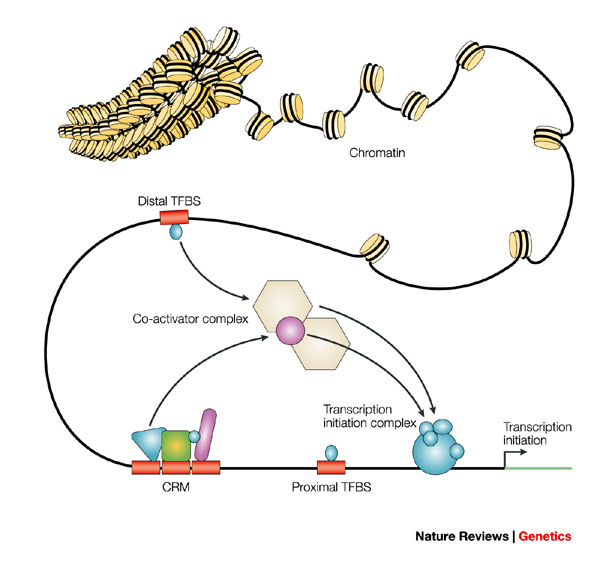
\includegraphics[width=0.8\linewidth]{images/crm.jpg}
  \end{figure}
\end{frame}
}

\begin{frame}[fragile]{TFBS: Properties}
  \begin{columns}[T,onlytextwidth]
    \column{0.5\textwidth}
    \begin{itemize}[<+- | alert@+>]
    	\item Short sequences (5-25bp)
  	  	\item Proximity to TSS (~100-1000bp)
   		\item Degeneracy
        %\item Under selection
    \end{itemize}
	\column{0.5\textwidth}
	\begin{texshade}{images/aln-msf.txt}
      \setends{1}{1..5}
      \hidenumbering
      \showsequencelogo{top}
      \showconsensus[ColdHot]{bottom}
      \defconsensus{.}{lower}{upper}
	\end{texshade}
  \end{columns}
\end{frame}

\begin{frame}[fragile]{Motif Discovery : Available Information}
  \begin{columns}[T,onlytextwidth]
    \column{0.5\textwidth}
		Two available axes of information:
      \begin{itemize}[<+- | alert@+>]
     	 \item Over-representation
    	 \item Cross-specie conservation
      \end{itemize}
    \column{0.5\textwidth}
    \begin{figure}
    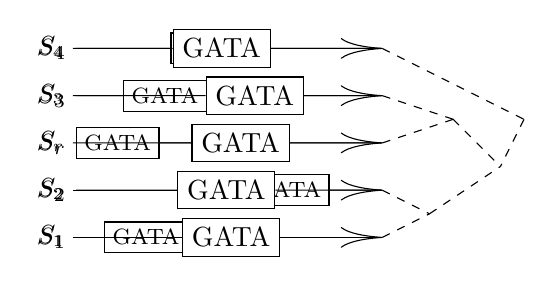
\begin{tikzpicture}[scale=0.6]
    \uncover<1>{\footnotesize
    \tikzstyle{operator} = [draw,fill=white,minimum size=1em] 
    \node at (0,0) (q1) {$S_1$};
    \node at (0,1) (q2) {$S_2$};
    \node at (0,2) (qr) {$S_r$};
    \node at (0,3) (q3) {$S_3$};
    \node at (0,4) (q4) {$S_4$};

    \node[operator] (op11) at (2,0) {GATA} edge [-] (q1);
    \draw[-{>[scale=2.5,
    length=6,
    width=3]}](op11) -- (7,0);

    \node[operator] (op21) at (5,1) {GATA} edge [-] (q2);
    \draw[-{>[scale=2.5,
    length=6,
    width=3]}] (op21) -- (7,1);

    \node[operator] (opr1) at (1.4,2) {GATA} edge [-] (qr);
    \draw[-{>[scale=2.5,
    length=6,
    width=3]}](opr1) -- (7,2);

    \node[operator] (op31) at (2.4,3) {GATA} edge [-] (q3);
    \draw[-{>[scale=2.5,
    length=6,
    width=3]}] (op31) -- (7,3);

    \node[operator] (op41) at (3.4,4) {GATA} edge [-] (q4);
    \draw[-{>[scale=2.5,
    length=6,
    width=3]}] (op41) -- (7,4);
   }
   \uncover<2->{
    \tikzstyle{operator} = [draw,fill=white,minimum size=1em] 
    \node at (0,0) (q1) {$S_1$};
    \node at (0,1) (q2) {$S_2$};
    \node at (0,2) (qr) {$S_r$};
    \node at (0,3) (q3) {$S_3$};
    \node at (0,4) (q4) {$S_4$};
        
    \node[operator] (op11) at (3.8,0) {GATA} edge [-] (q1);
    \draw(op11) -- (7,0);
    \draw[dashed](7,0) -- (8,0.5);
    \draw[dashed](8,0.5) -- (9.5, 1.5);

    \node[operator] (op21) at (3.7,1) {GATA} edge [-] (q2);
    \draw (op21) -- (7,1);
    \draw[dashed](7,1) -- (8,0.5);

    \node[operator] (opr1) at (4,2) {GATA} edge [-] (qr);
    \draw(opr1) -- (7,2);
    \draw[dashed](7,2) -- (8.5,2.5);
    
    \node[operator] (op31) at (4.3,3) {GATA} edge [-] (q3);
    \draw(op31) -- (7,3);
    \draw[dashed](7,3) -- (8.5,2.5);
    \draw[dashed](8.5,2.5) -- (9.5, 1.5);

    \node[operator] (op41) at (3.6,4) {GATA} edge [-] (q4);
    \draw(op41) -- (7,4);
    \draw[dashed](7,4) -- (10, 2.5);
	\draw[dashed](10,2.5) -- (9.5,1.5);    
    }
   \end{tikzpicture}
     \end{figure}
    
  \end{columns}
\end{frame}

\begin{comment}
\begin{frame}[fragile]{`Heterogenous data' and motif finding}
 \begin{columns}[T,onlytextwidth]
    \column{0.5\textwidth}
	  \begin{itemize}
      \item `Heterogeneity' -- sequences from co-regulated genes or orthologous regions
      \item Assumption of independent sequences does not hold
      \item Need to account for phylogenetic relationships
      \item \textbf{Key Idea:} Functional sequences evolve slower than non-functional ones
      \end{itemize}
      \column{0.5\textwidth}
\footnotesize
\begin{figure}
    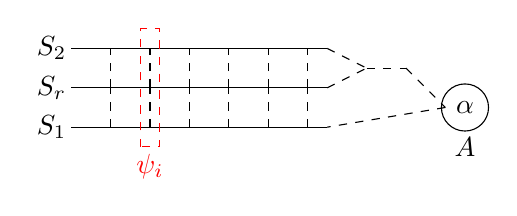
\begin{tikzpicture}[scale=0.5]
    \node at (0,0) (q1) {$S_1$};
    \node at (0,1) (q2) {$S_r$};    
    \node at (0,2) (q3) {$S_2$};    
        
    \draw (0.5,0) -- (7,0);
    \draw (0.5,1) -- (7,1);
    \draw (0.5,2) -- (7,2);
    \draw[dashed] (1.5,0) -- (1.5,1);
    \draw[dashed] (2.5,0) -- (2.5,1);
    \draw[dashed] (3.5,0) -- (3.5,1);
    \draw[dashed] (4.5,0) -- (4.5,1);
    \draw[dashed] (5.5,0) -- (5.5,1);
    \draw[dashed] (6.5,0) -- (6.5,1);
    
    \draw[dashed] (1.5,1) -- (1.5,2);
    \draw[dashed] (2.5,1) -- (2.5,2);
    \draw[dashed] (3.5,1) -- (3.5,2);
    \draw[dashed] (4.5,1) -- (4.5,2);
    \draw[dashed] (5.5,1) -- (5.5,2);
    \draw[dashed] (6.5,1) -- (6.5,2);
    
	\draw[dashed, red] (2.25,-0.5) rectangle (2.75,2.5);
    \node[red] at (2.5, -1) (q4) {$\psi_i$};
    
    \draw[dashed](7,2) -- (8,1.5);
    \draw[dashed](7,1) -- (8,1.5);
    \draw[dashed](8,1.5) -- (9,1.5);
    \draw[dashed](9,1.5) -- (10,0.5);
    \draw[dashed](10,0.5) -- (7,0);
    
    \node[circle, draw] at (10.5,0.5) {$\alpha$};
    \node at (10.5, -0.5) {$A$};
\end{tikzpicture}
\caption{\footnotesize MSA of Orthologous Sequences}
\end{figure}
  \end{columns}
   \begin{columns}[T,onlytextwidth]
    \column{0.5\textwidth}
      \begin{align*}       
        P(\psi_i) &= \sum_{\alpha }P(\psi_i, A_i=\alpha | \theta)\\  
        &= \sum_\alpha P(A_i=\alpha)P(\psi_i| A_i=\alpha,\theta) \\ 
        &= \sum_\alpha P(A_i=\alpha)\prod_{s_i}\highlight{P(s_i| A_i=\alpha,\theta) }\\ 
        %&= \sum_{\alpha} \theta_{i\alpha}\prod_{k=1}^K P_{\alpha s_{i}^k}\\
      \end{align*}
      \column{0.5\textwidth}
      \begin{align*}
      S &= \{\psi_1, \psi_2, \dots, \psi_L\};\\
		\theta_{i\alpha} &= \text{$i^{th}$ PWM entry for base $\alpha$}\\
        P_{\alpha S_i^k} &= \text{$k^{th}$ base of $i^{th}$ sequence}
		\end{align*}
 	 \end{columns}
\end{frame}
\end{comment}

\begin{frame}[fragile]{`Heterogenous data' and motif finding}
	  \begin{itemize}
      \item `Heterogeneity' -- sequences from co-regulated genes or orthologous regions
      \item Assumption of independent sequences does not hold
      \item Need to account for phylogenetic relationships
      \item \textbf{Key Idea:} Functional sequences evolve slower than non-functional ones
      \end{itemize}
\end{frame}

\begin{frame}[fragile]{General Model for evolutionary approaches}
\footnotesize
\begin{figure}
    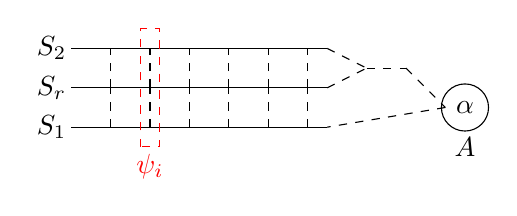
\begin{tikzpicture}[scale=0.5]
    \node at (0,0) (q1) {$S_1$};
    \node at (0,1) (q2) {$S_r$};    
    \node at (0,2) (q3) {$S_2$};    
        
    \draw (0.5,0) -- (7,0);
    \draw (0.5,1) -- (7,1);
    \draw (0.5,2) -- (7,2);
    \draw[dashed] (1.5,0) -- (1.5,1);
    \draw[dashed] (2.5,0) -- (2.5,1);
    \draw[dashed] (3.5,0) -- (3.5,1);
    \draw[dashed] (4.5,0) -- (4.5,1);
    \draw[dashed] (5.5,0) -- (5.5,1);
    \draw[dashed] (6.5,0) -- (6.5,1);
    
    \draw[dashed] (1.5,1) -- (1.5,2);
    \draw[dashed] (2.5,1) -- (2.5,2);
    \draw[dashed] (3.5,1) -- (3.5,2);
    \draw[dashed] (4.5,1) -- (4.5,2);
    \draw[dashed] (5.5,1) -- (5.5,2);
    \draw[dashed] (6.5,1) -- (6.5,2);
    
	\draw[dashed, red] (2.25,-0.5) rectangle (2.75,2.5);
    \node[red] at (2.5, -1) (q4) {$\psi_i$};
    
    \draw[dashed](7,2) -- (8,1.5);
    \draw[dashed](7,1) -- (8,1.5);
    \draw[dashed](8,1.5) -- (9,1.5);
    \draw[dashed](9,1.5) -- (10,0.5);
    \draw[dashed](10,0.5) -- (7,0);
    
    \node[circle, draw] at (10.5,0.5) {$\alpha$};
    \node at (10.5, -0.5) {$A$};
\end{tikzpicture}
\caption{\footnotesize MSA of Orthologous Sequences}
\end{figure}
   \begin{columns}[T,onlytextwidth]
    \column{0.5\textwidth}
      \begin{align*}       
        P(\psi_i) &= \sum_{\alpha }P(\psi_i, A_i=\alpha | \theta)\\  
        &= \sum_\alpha P(A_i=\alpha)P(\psi_i| A_i=\alpha,\theta) \\ 
        &= \sum_\alpha P(A_i=\alpha)\prod_{s_i}\highlight{P(s_i| A_i=\alpha,\theta) }\\ 
        %&= \sum_{\alpha} \theta_{i\alpha}\prod_{k=1}^K P_{\alpha s_{i}^k}\\
      \end{align*}
      \column{0.5\textwidth}
      \begin{align*}
    	S &= \{\psi_1, \psi_2, \dots, \psi_L\};\\
        A &= \text{Unobserved ancestral sequence}\\
		\theta_{i\alpha} &= \text{$i^{th}$ PWM entry for base $\alpha$}\\
        P_{\alpha S_i^k} &= \text{$k^{th}$ base of $i^{th}$ sequence}
		\end{align*}
 	 \end{columns}

\end{frame}

\begin{frame}[fragile]{Substitution Models}
\begin{itemize}
\item Evolution can be modeled as a continuous time markov chain: $\mathbf{P}(t) = (P_{ij}(t))$
\item $P'(t) = QP(t)$, where $Q$ is the mutation rate matrix 
\item $Q= \begin{pmatrix} * & \mu_{AC} & \mu_{AG} & \mu_{AT}\\
& & \cdots \end{pmatrix}$
\item Simple models 
\begin{itemize}
\item Jukes Cantor (JC69): Equal base frequencies $\pi_A = \pi_G = \pi_C = \pi_T$
\item Kimura (K80): Distinguishes between transition and transversion ratios
\item Felenstein (F81): Allows different base frequencies
\end{itemize} 
\end{itemize} 
\end{frame}

\begin{comment}
\begin{frame}[fragile]{Model Assumptions}
\begin{itemize}
\item Probability of fixation of a mutation $\alpha \rightarrow \beta$ is proportional to corresponding PWM entry. ($P(A_i=\alpha) = \theta_{i\alpha}$)
\item $P(s_i|A_i)$ is determined by using different substitution models which is our focus here
\end{itemize}
\end{frame}
\end{comment}


\begin{frame}[fragile]{Halpern Bruno Model : Accounting for Selection }
\begin{itemize}
\item `Selection aware' substitution model, original formulated for coding-sequence
\item All positions in the binding site evolve independently at equal rates
%\item Besides accounting for difference in equilbrium frequencies, it is also important to account for selection
\item Effect of selection applies on probabilities of fixation once a mutation has occurred
\item Fixation is rapid, allowing no time for polymorphism to exist
%\item Each base position evolves independently
\item Only negative selection acts
\item Covariation structure between different species are ignored
\item \textbf{Key Insight} Grater the difference in fitness ($f_{\alpha\beta}$) less overall substitution
%\item F81 considers evolutionary distance ignoring selection pressure
\end{itemize}
\end{frame}


\begin{frame}[fragile]{Halpern Bruno Model : Accounting for Selection}
\begin{align*}
r_{\alpha\beta}^i &= \text{Rate at which base $\alpha$ is replaced by $\beta$}\\
p_{\alpha\beta} &= \text{Site invariant probability of mutation}\\
f_{\alpha\beta}^i &= \text{Site specific probability of fixation}\\
r_{\alpha\beta}^i &= p_{\alpha\beta} \times f_{\alpha\beta}^i\\
r_{\alpha\alpha}^i &= -\sum_{\beta, \beta \neq \alpha} r_{\alpha\beta}^i
\end{align*}
\begin{itemize}
\item Kimura's fixation probability: $f_{\alpha\beta} = \frac{1-e^{-s}}{1-e^{-2Ns}}$ where fitness = $1+s$, $s<<1$
\item No polymorphism approximation: $f_{\alpha\beta} \approx \frac{2s}{1-e^{-2Ns}}$, $f_{\beta\alpha} \approx \frac{-2s}{1-e^{2Ns}}$
\item Reversibility condition: $\pi_\alpha p_{\alpha\beta}f_{\alpha\beta} = \pi_\beta p_{\beta\alpha} f_{\beta\alpha} \implies \frac{\pi_\beta f_{\beta\alpha}}{\pi_\alpha f_{\alpha\beta}} = \frac{f_{\alpha\beta}}{f_{\beta\alpha}} = e^{2Ns} $\\
\item $f_{\alpha\beta} \propto \frac{\ ln{\frac{\pi_\beta p_{\beta\alpha}  }{ \pi_\alpha p_{\alpha_\beta} } }} 
{1- \frac{ \pi_\alpha p_{\alpha_\beta} } {\pi_\beta p_{\beta\alpha} } } $  $\implies r_{\alpha\beta} = p_{\alpha\beta} \frac{\ln{\frac{\pi_\beta p_{\beta\alpha}}{\pi_\alpha p_{\alpha\beta}}}}{1-\frac{\pi_\alpha p_{\alpha\beta}  }{\pi_\alpha p_{\beta\alpha}  } } $
\item $P(t) = \exp(r_{\alpha\beta} t)$
\end{itemize}
\end{frame}


\begin{frame}[fragile]{Lineage specific evolution}
   \begin{columns}[T,onlytextwidth]
    \column{0.5\textwidth}
    \begin{figure}
		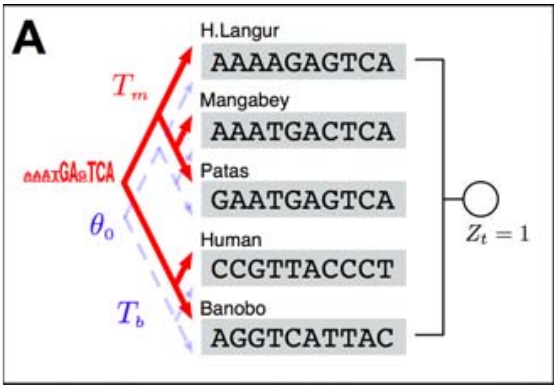
\includegraphics[width=0.77\textwidth]{images/monkey-model.png}
        \caption{Modeling full phylogeny as one component}
	\end{figure}
    \column{0.5\textwidth}
    \uncover<2>{\begin{figure}
		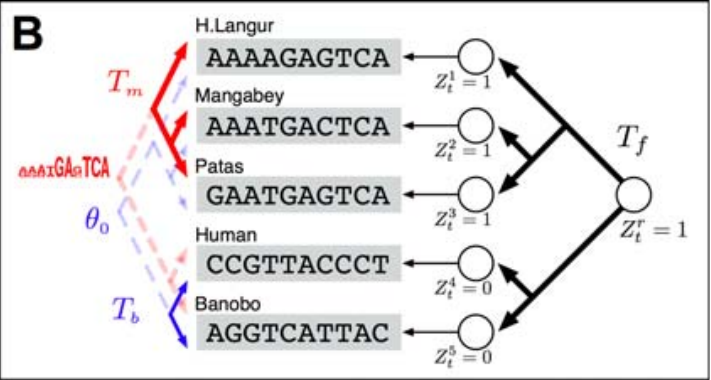
\includegraphics[width=\textwidth]{images/csmet-model.png}
        \caption{Modeling full phylogeny as one component}
	\end{figure}}
    \end{columns}
\end{frame}

\begin{frame}[fragile]{Ornstein-Uhlenbeck Models: Whole TFBS evolving as a unit}
\begin{itemize}
\item HB models neglects lineage or specie specific selection
\item OU models this gap by accounting for lineage/specie specific selection by requiring regime specific optima to be obtained
\item OU models can account for whole element substituion by defining a quantitative trait as a score attached to the TFBS $X(t)$
\item $X(t)$ evolves by two components one deterministic, other stochastic (BM)
\end{itemize}
\begin{align*}
dX(t) &= \alpha(\theta-X(t)) + \sigma dB(t)\\
\alpha & = \text{Strength of selection}\\
\theta - X(t) & = \text{Distance from optimum value}\\
\sigma &= \text{strength of random drift}\\
dB(t) &= \text{random white noise}
\end{align*}
\end{frame}


\begin{frame}[fragile]{Selection acts on whole site?}
\begin{itemize}
\item Susbtitution rates are position specific in TFBS but independence assumption does not necessarily hold
\item Intuition: A TFBS will retain functionality if it is close enough to optimality even if a single nucleotide undergoes substitution eventually getting fixed
\item The same substituion in a far less optimal site might lead to a functional loss
\item A better model would be to account for substitution of entire site i.e. site-level selection treating bindinig sites as evolutionary units
%\item Each site can take two fitness values: $1$ or $1+s$ where the former refers to equally fit substitution and the latter implies a substandard substitution
%\item The site is functional if it is below a certain energy threshold (bindin
\end{itemize}
\end{frame}

\begin{frame}[fragile]{Ornstein-Uhlenbeck Models: Whole TFBS evolving as a unit}
   \begin{columns}[T,onlytextwidth]
    \column{0.3\textwidth}
	\begin{figure}
    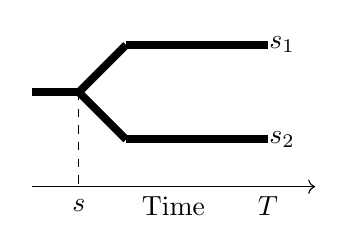
\begin{tikzpicture}[scale=0.6]
    \tikzstyle{operator} = [draw,fill=white,minimum size=1em] 
        \draw[->] (0,-2) -- (6,-2);
        \draw[line width=1mm] (0,0) -- (1,0);   
        \draw[line width=1mm] (1,0) -- (2,1);
        \draw[line width=1mm] (2,1) -- (5,1);
        \draw[line width=1mm] (1,0) -- (2,-1);
        \draw[line width=1mm] (2,-1) -- (5,-1);   
        \draw[dashed] (1,0) -- (1,-2);
        \node at (1,-2.4) {$s$};
        \node at (3,-2.4) {Time};
        \node at (5,-2.4) {$T$};
        \node at (5.3,1) {$s_1$};
        \node at (5.3,-1) {$s_2$};
    \end{tikzpicture}
\caption{$s_1$, $s_2$ -- BM}    
\end{figure}

	\column{0.7\textwidth}    
    \begin{align*}
E[\mathbf{X}(t)] &= \begin{pmatrix}
\theta_0\\
\theta_1
\end{pmatrix}\\
 \texorpdfstring{{\Sigma}} &= \sigma^2\begin{pmatrix}
T & s\\
s & T
\end{pmatrix}\\
\end{align*}    
  \end{columns}
  \begin{columns}[T,onlytextwidth]
    \column{0.3\textwidth}     
    \begin{figure}
    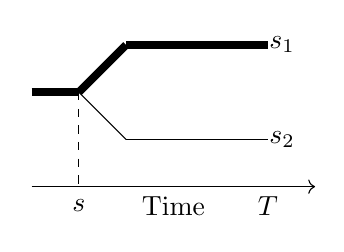
\begin{tikzpicture}[scale=0.6]
    \tikzstyle{operator} = [draw,fill=white,minimum size=1em] 
        \draw[->] (0,-2) -- (6,-2);
        \draw[line width=1mm] (0,0) -- (1,0);   
        \draw[line width=1mm] (1,0) -- (2,1);
        \draw[line width=1mm] (2,1) -- (5,1);
        \draw (1,0) -- (2,-1);
        \draw (2,-1) -- (5,-1);   
        \draw[dashed] (1,0) -- (1,-2);
        \node at (1,-2.4) {$s$};
        \node at (3,-2.4) {Time};
        \node at (5,-2.4) {$T$};
        \node at (5.3,1) {$s_1$};
        \node at (5.3,-1) {$s_2$};
    \end{tikzpicture}
    \caption{$s_2$ -- new optimum regime, $s_1$ -- ancestral}    
\end{figure}
    \column{0.7\textwidth}
    \begin{align*}
      E[X_1(T)] &= \theta_0e^{-\alpha T}+ \theta_1(1-e^{-\alpha T})\\
      E[X_2(T)] &= \theta_0e^{-\alpha T} + \theta_1e^{-\alpha(T-s)}(1-e^{-\alpha s})\\ 
      &+ \theta_2(1-e^{-\alpha(T-s)})\
	\end{align*}
  \end{columns}
\end{frame}

\begin{frame}[fragile]{Turnovers}
\begin{figure}
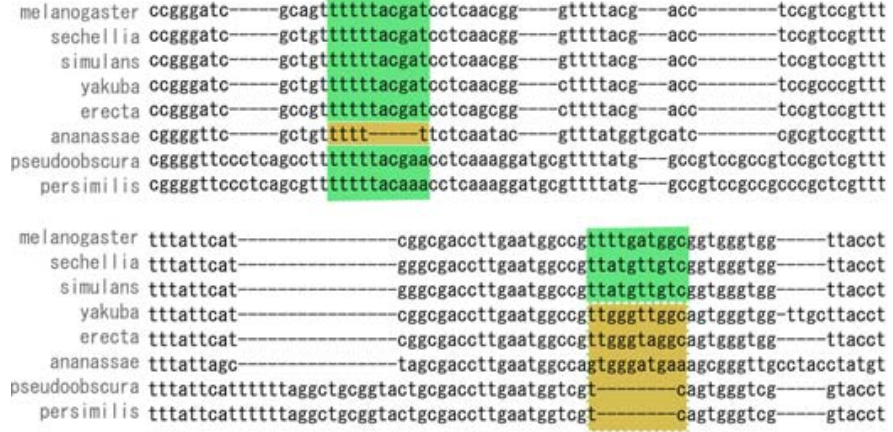
\includegraphics[width=\textwidth]{images/turnover}
\caption{Functional turnover: TFBS can be gained or lost during evolution}
\end{figure}
\end{frame}

\begin{frame}[fragile]{Functional turnover: Birth \& Death Process}
Aim: Detect lineage-specific rates of TFBS evolution and the branch of origin of individual TFBS
\begin{itemize}
\item Binding sites are known to show turnover: TFBS can be gained/lost during speciation events 
\item Estimate rate of birth $\alpha$ and death $\beta$ from orthologous sequences
\item In contrast to conservation based approaches, use birth-death model to infer ancestral states
\end{itemize}
\end{frame} 

\begin{frame}[fragile]{Functional turnover: Birth \& Death Process}
\begin{align*}
w(t) &= \text{Probability that TFBS exists time $t$}\\
\alpha,\beta &= \text{Birth, death rate respectively}\\
w(t+1) &= \alpha(1-w(t)) + (1-\beta) w(t)\\
w'(t) &= \alpha - (\alpha+\beta) w(t)
\end{align*}

We formulate two type of solutions, $u(t), v(t)$ such that $u(t)$ represents those class of motifs present at $t=0$
and $v(t)$ represents class of motifs that did not exist at $t=0$.
\end{frame} 

\begin{frame}[fragile]{Functional turnover: Birth \& Death Process}
Let $p_{ij}(t)$ represent the probability of observing $j$ motif occurrences after $t$ , initial $i$
\begin{align*}
u(t) &= \frac{1}{\alpha+\beta} (\alpha + \beta e^{-(\alpha+\beta)t})\\
v(t) &= \frac{\alpha}{\alpha+\beta} (1-e^{-(\alpha+\beta)t})\\
U_{i,k}(t) &= \frac{i!}{(i-k)!k!}{u(t)}^k(1-u(t))^k\\
V_{N-i,b}(t) &= \frac{(N-i)!}{(N-i-b)!b!} {v(t)}^b (1-v(t))^{N-i-b}\\
p_{i,j}(t) &= \sum_{k=0}^{\min{i,j}} U_{i,k}(t) V_{N-i,j-k}(t)
\end{align*}
\end{frame} 






\begin{comment}


\begin{frame}[fragile]{Problem with Phylogenetic Shadowing based approaches}
\begin{itemize}
\item Two main assumptions on approaches so far:
\begin{itemize}
\item Independence: Sites evolve independently
\item Completeness: Orthology as captured by MSA complete
\end{itemize}
\item Unlike genes, TFBS exhibit frequent turnover 
\end{itemize}
Assumptions make modeling easier, works well for gene coding regions in closesly related taxa since in genes turnover 
PhyME, MONKEY do not offer any insight into evolutionars dyanmics of motif turnover.
\end{frame}
\end{comment}




\begin{comment}
\begin{frame}[fragile]{Birth-Death model: Where's the branch}
\begin{figure}
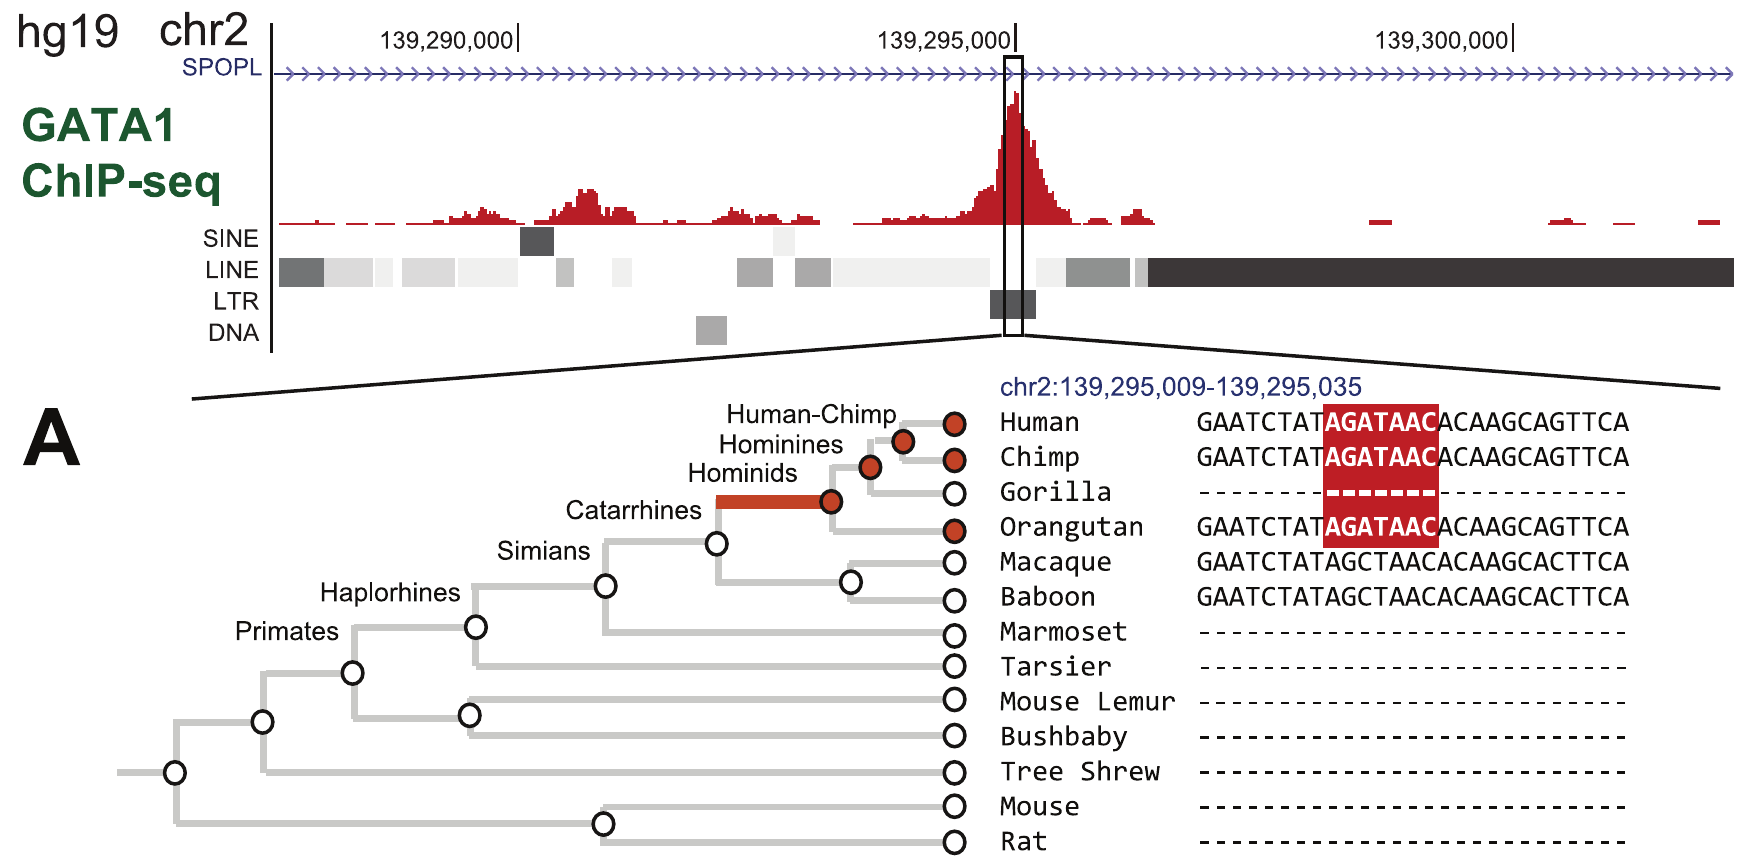
\includegraphics[width=\linewidth]{images/branchorigin.png}
\caption{Phylogenies in the birth-death model framewrok}
\end{figure}

\end{frame}
\end{comment}





\begin{frame}[fragile]{Lineage Specific: CSMET}
\begin{figure}
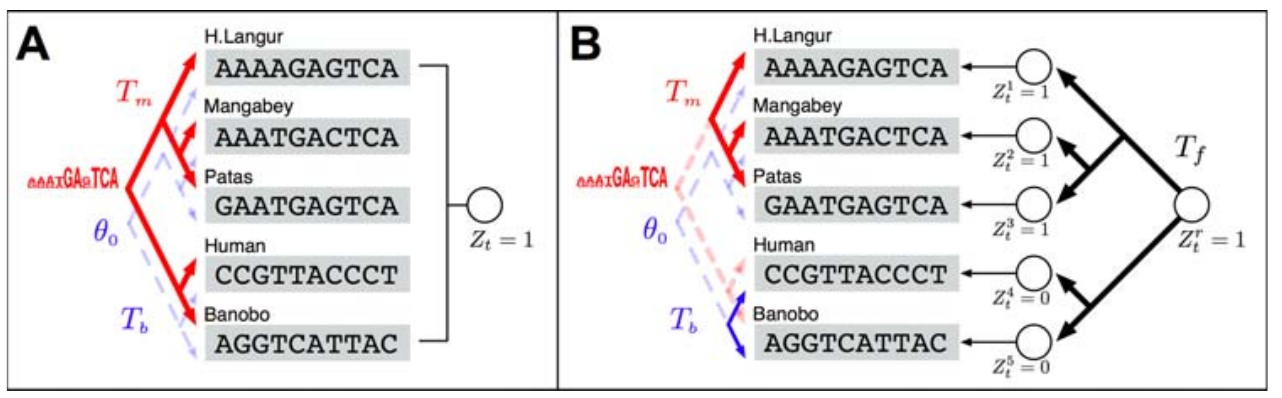
\includegraphics[width=\linewidth]{images/csmet1.png}
\caption{A) Modeling full phylogeny as one component mixture B) Lieange specific model}
\end{figure}
\end{frame}

\begin{frame}[fragile]{Lineage Specific: CSMET}
\begin{figure}
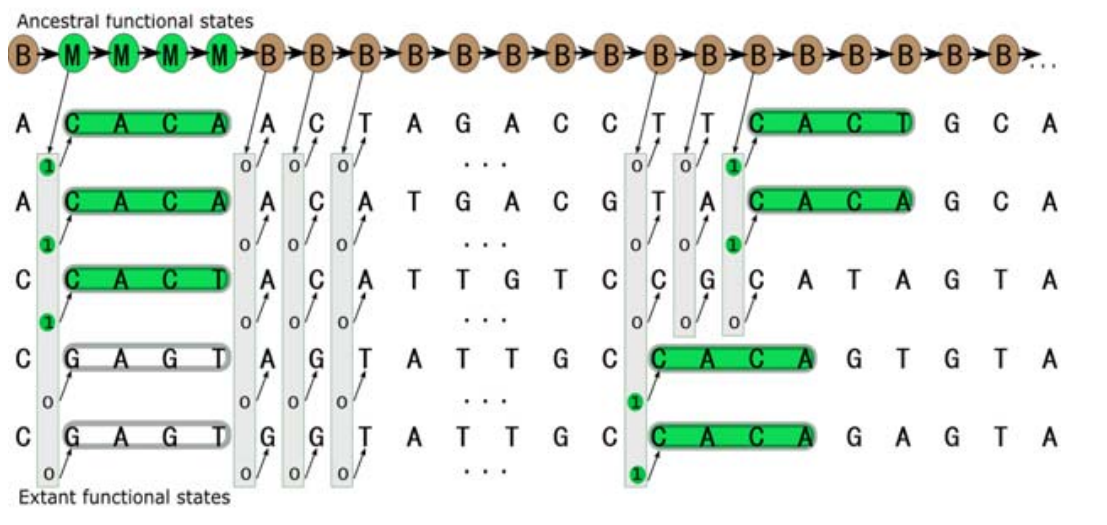
\includegraphics[width=\linewidth]{images/csmet2.png}
\caption{Ancestor background - evolution independent, Ancestor motif TFBS evolves as unit}
\end{figure}
\end{frame}

\begin{frame}[fragile]{Lineage Specific: CSMET}
\begin{itemize}
\item 
\end{itemize}
\end{frame}


\begin{frame}{Summary}
Summary
\end{frame}

\begin{frame}[standout]
  Questions?
\end{frame}

\appendix



\end{document}
